\chapter{Security Challenges in Smart Constracts}
\markboth{Title of My Seminar Work}{}
\chaptauthors{Lucas Pelloni and Ile Cepilov}

\Kurzfassung{%
This is the abstract.
It fits pretty much on one page and is definitely not longer.}

\newpage

\minitoc %table of contents

\newpage

%http://blockgeeks.com/guides/what-is-blockchain-technology/
\section{What is Blockchain Technology?}
       \begin{figure}[ht]
         \begin{center}
         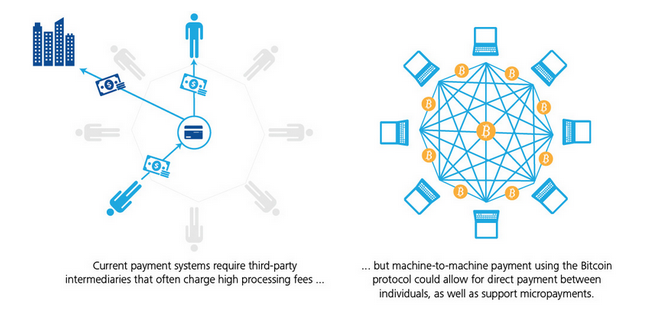
\includegraphics[scale=0.6]{Talk3/blockchain}
         \end{center}
         \caption{This is a pic FROM ILIA}
         \label{label}
       \end{figure}
       
\subsection{Blockchain and Bitcoins}
\subsection{A Distributed Database}
\subsection{How does it work?}

%https://letstalkpayments.com/an-overview-of-blockchain-technology

\section{What is a Smart Contract?}
%definition founded here: https://www.youtube.com/watch?v=FkeLDPZ-v8g&t=134s
A Smart Contract is a piece of software that stores rules for negotiating the terms of a contract, automatically verifies the contract and then executes the agreed terms. 


You only applhasfbihasbhofahisvfashivfasi